\documentclass[compress]{beamer}
\usepackage{ifthen,verbatim}

\title{Validation of CSA07 1\_6\_4 AlCaRecoMu samples}
\author{Jim Pivarski, Alexei Safonov}
\institute{Texas A\&M University}
\date{ 5 October, 2007}

\newcommand{\isnote}{}
\xdefinecolor{lightyellow}{rgb}{1.,1.,0.25}
\xdefinecolor{darkblue}{rgb}{0.1,0.1,0.7}

%% Uncomment this to get annotations
%% \def\notes{\addtocounter{page}{-1}
%%            \renewcommand{\isnote}{*}
%% 	   \beamertemplateshadingbackground{lightyellow}{white}
%%            \begin{frame}
%%            \frametitle{Notes for the previous page (page \insertpagenumber)}
%%            \itemize}
%% \def\endnotes{\enditemize
%% 	      \end{frame}
%%               \beamertemplateshadingbackground{white}{white}
%%               \renewcommand{\isnote}{}}

%% Uncomment this to not get annotations
\def\notes{\comment}
\def\endnotes{\endcomment}

\setbeamertemplate{navigation symbols}{}
\setbeamertemplate{headline}{\includegraphics[height=1 cm]{../cmslogo} \hspace{0.1 cm} \includegraphics[height=1 cm]{../tamulogo} \hfill
\begin{minipage}{5.5 cm}
\vspace{-0.75 cm} \small
\begin{center}
\ifthenelse{\equal{\insertpagenumber}{1}}{}{\textcolor{blue}{\insertsection}}
\end{center}
\end{minipage} \hfill
\begin{minipage}{4.5 cm}
\vspace{-0.75 cm} \small
\begin{flushright}
\ifthenelse{\equal{\insertpagenumber}{1}}{}{Jim Pivarski \hspace{0.5 cm} \insertpagenumber\isnote/\pageref{numpages}}
\end{flushright}
\end{minipage}\mbox{\hspace{0.2 cm}}}

\begin{document}
\frame{\titlepage}

%% \begin{notes}
%% \item This is the annotated version of my talk.
%% \item If you want the version that I am presenting, download the one
%% labeled ``slides'' on Indico (or just ignore these yellow pages).
%% \item The annotated version is provided for extra detail and a written
%% record of comments that I intend to make orally.
%% \item Yellow notes refer to the content on the {\it previous} page.
%% \item All other slides are identical for the two versions.
%% \end{notes}

\section*{Validation of 1\_6\_4 AlCaRecoMu}

\begin{frame}
\small I'll get right to the plots!

\begin{center}
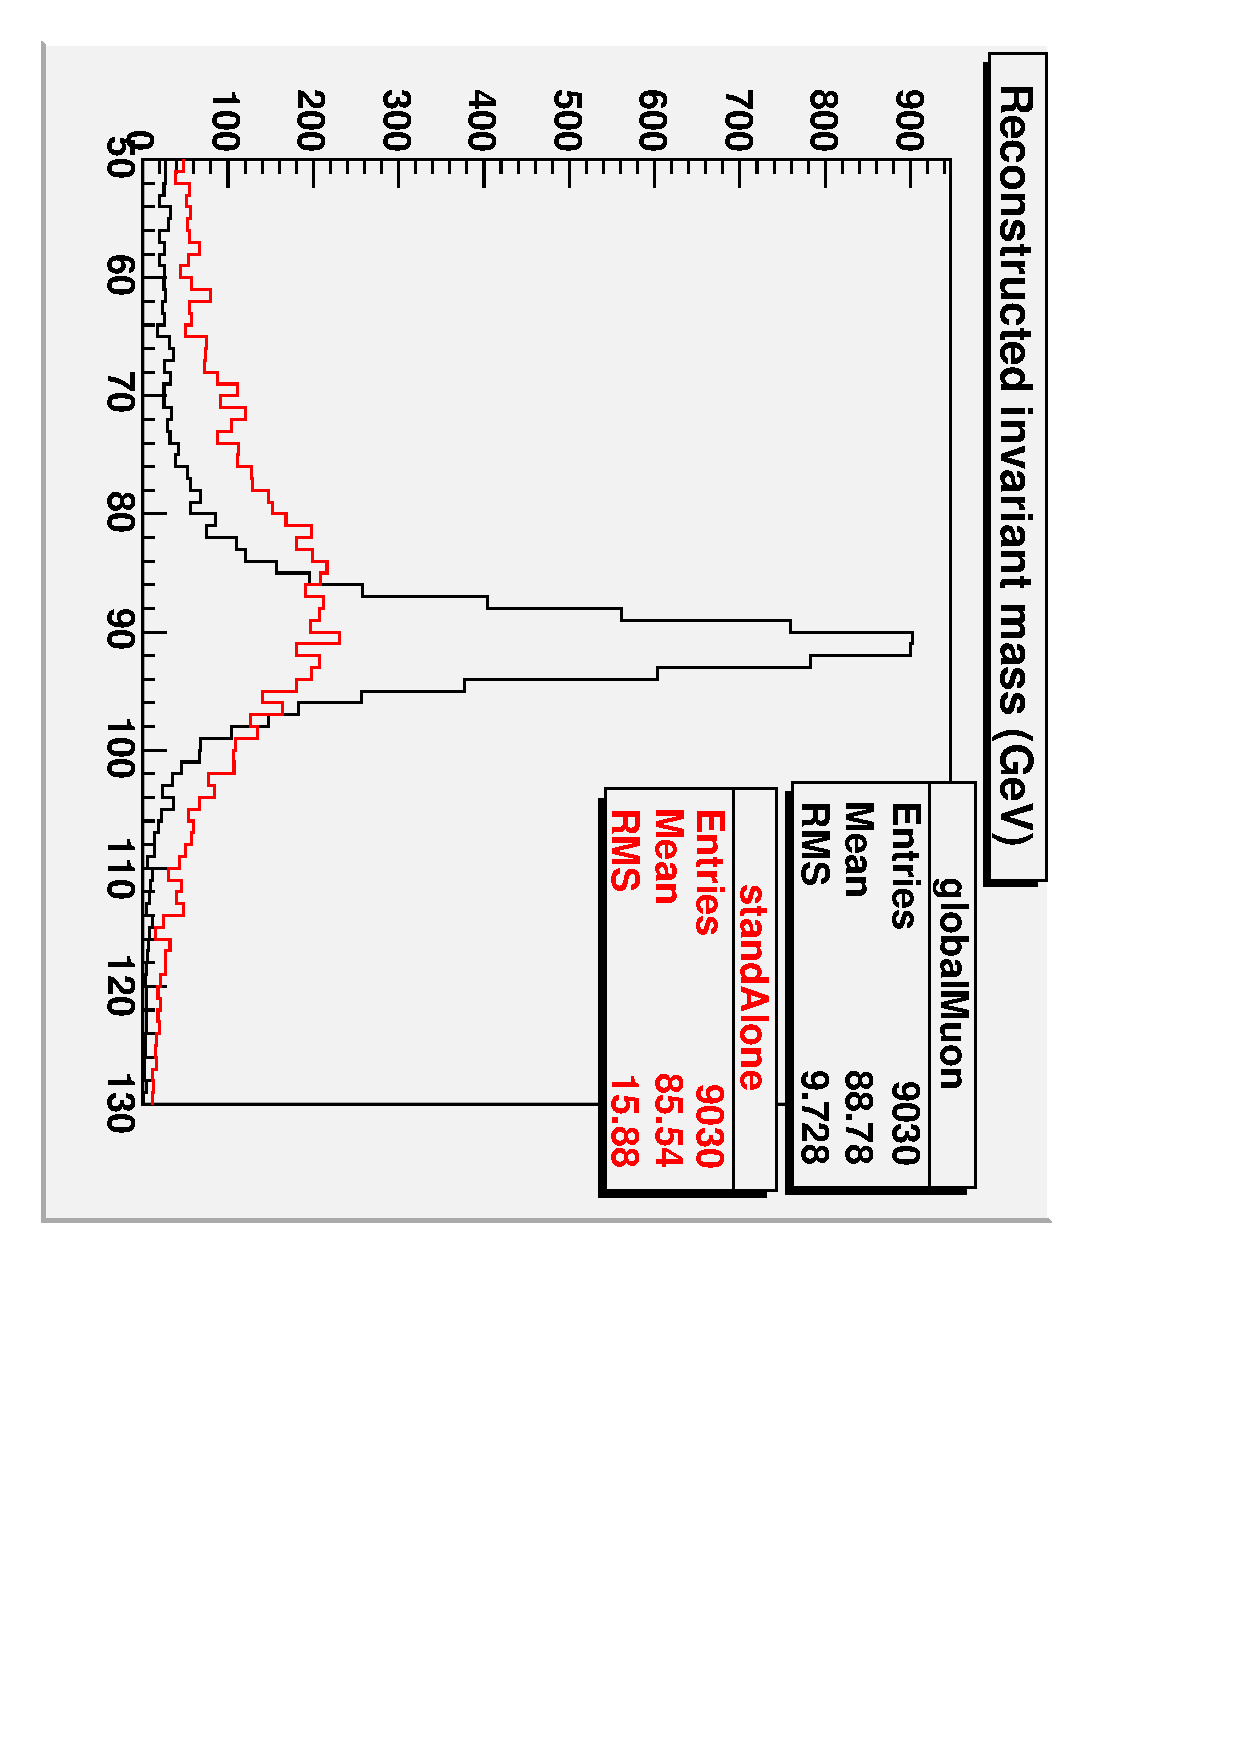
\includegraphics[width=5.5 cm, angle=90]{z_peaks.pdf}
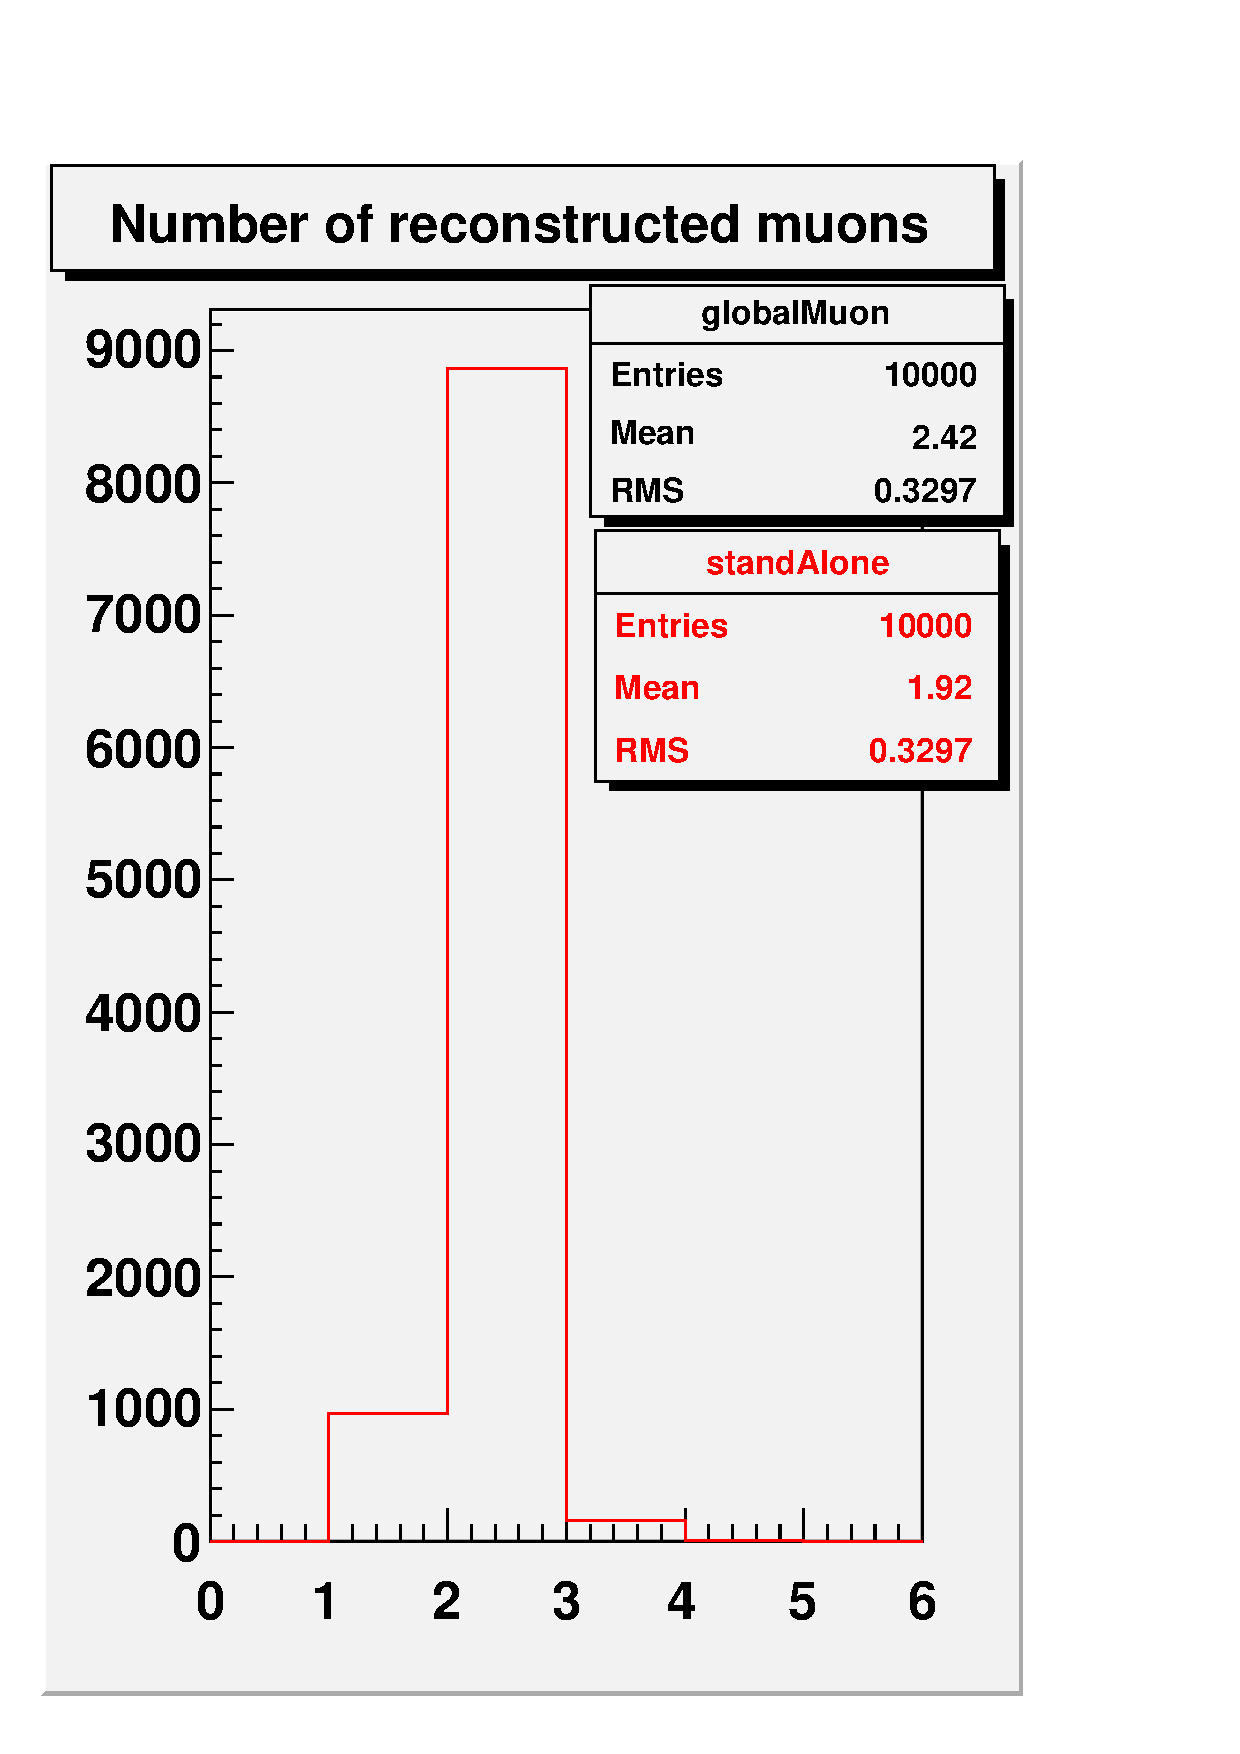
\includegraphics[height=5.5 cm]{nmuons.pdf}
\end{center}

These are all in 1\_6\_4: I could not compare with 1\_5\_4 because I
couldn't access my personal CASTOR\ldots?
\end{frame}

\begin{frame}
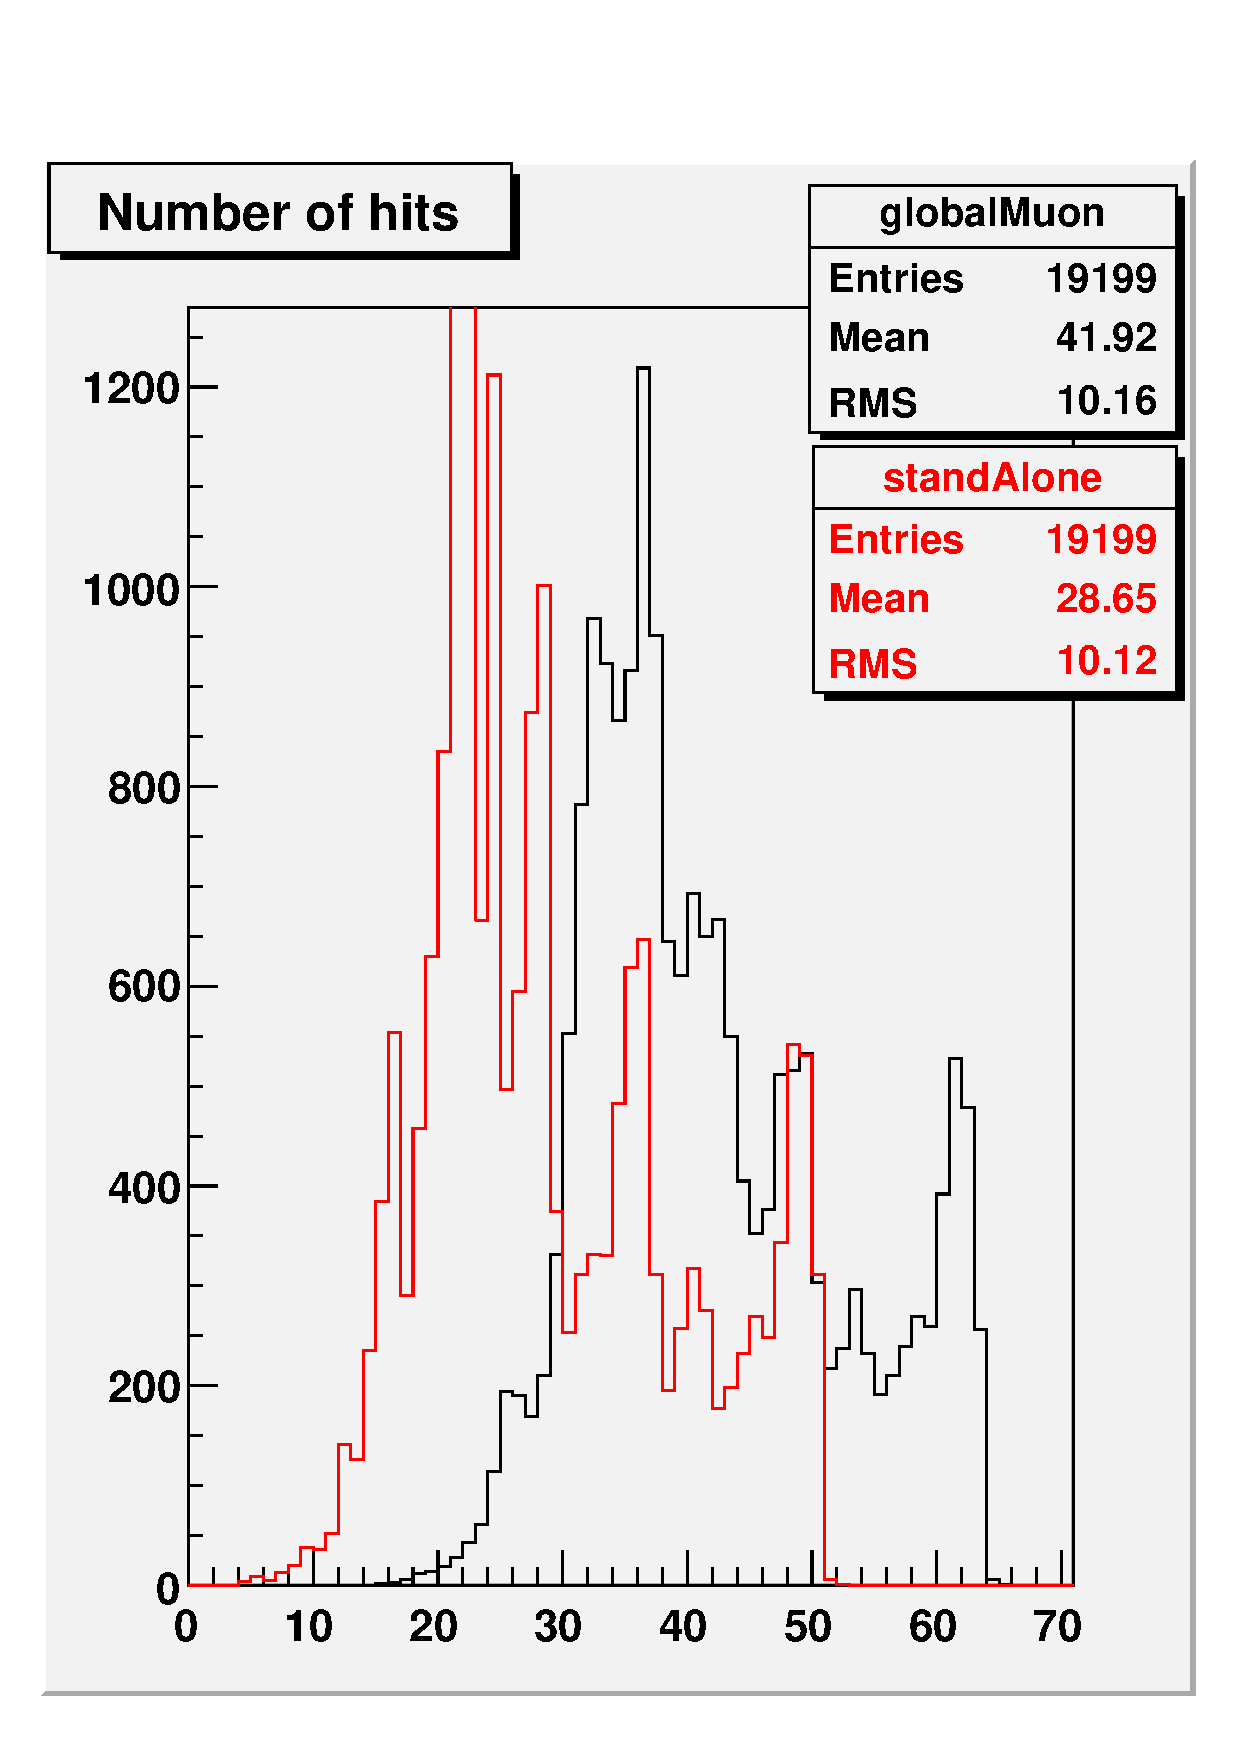
\includegraphics[width=0.5\linewidth]{nhits.pdf}
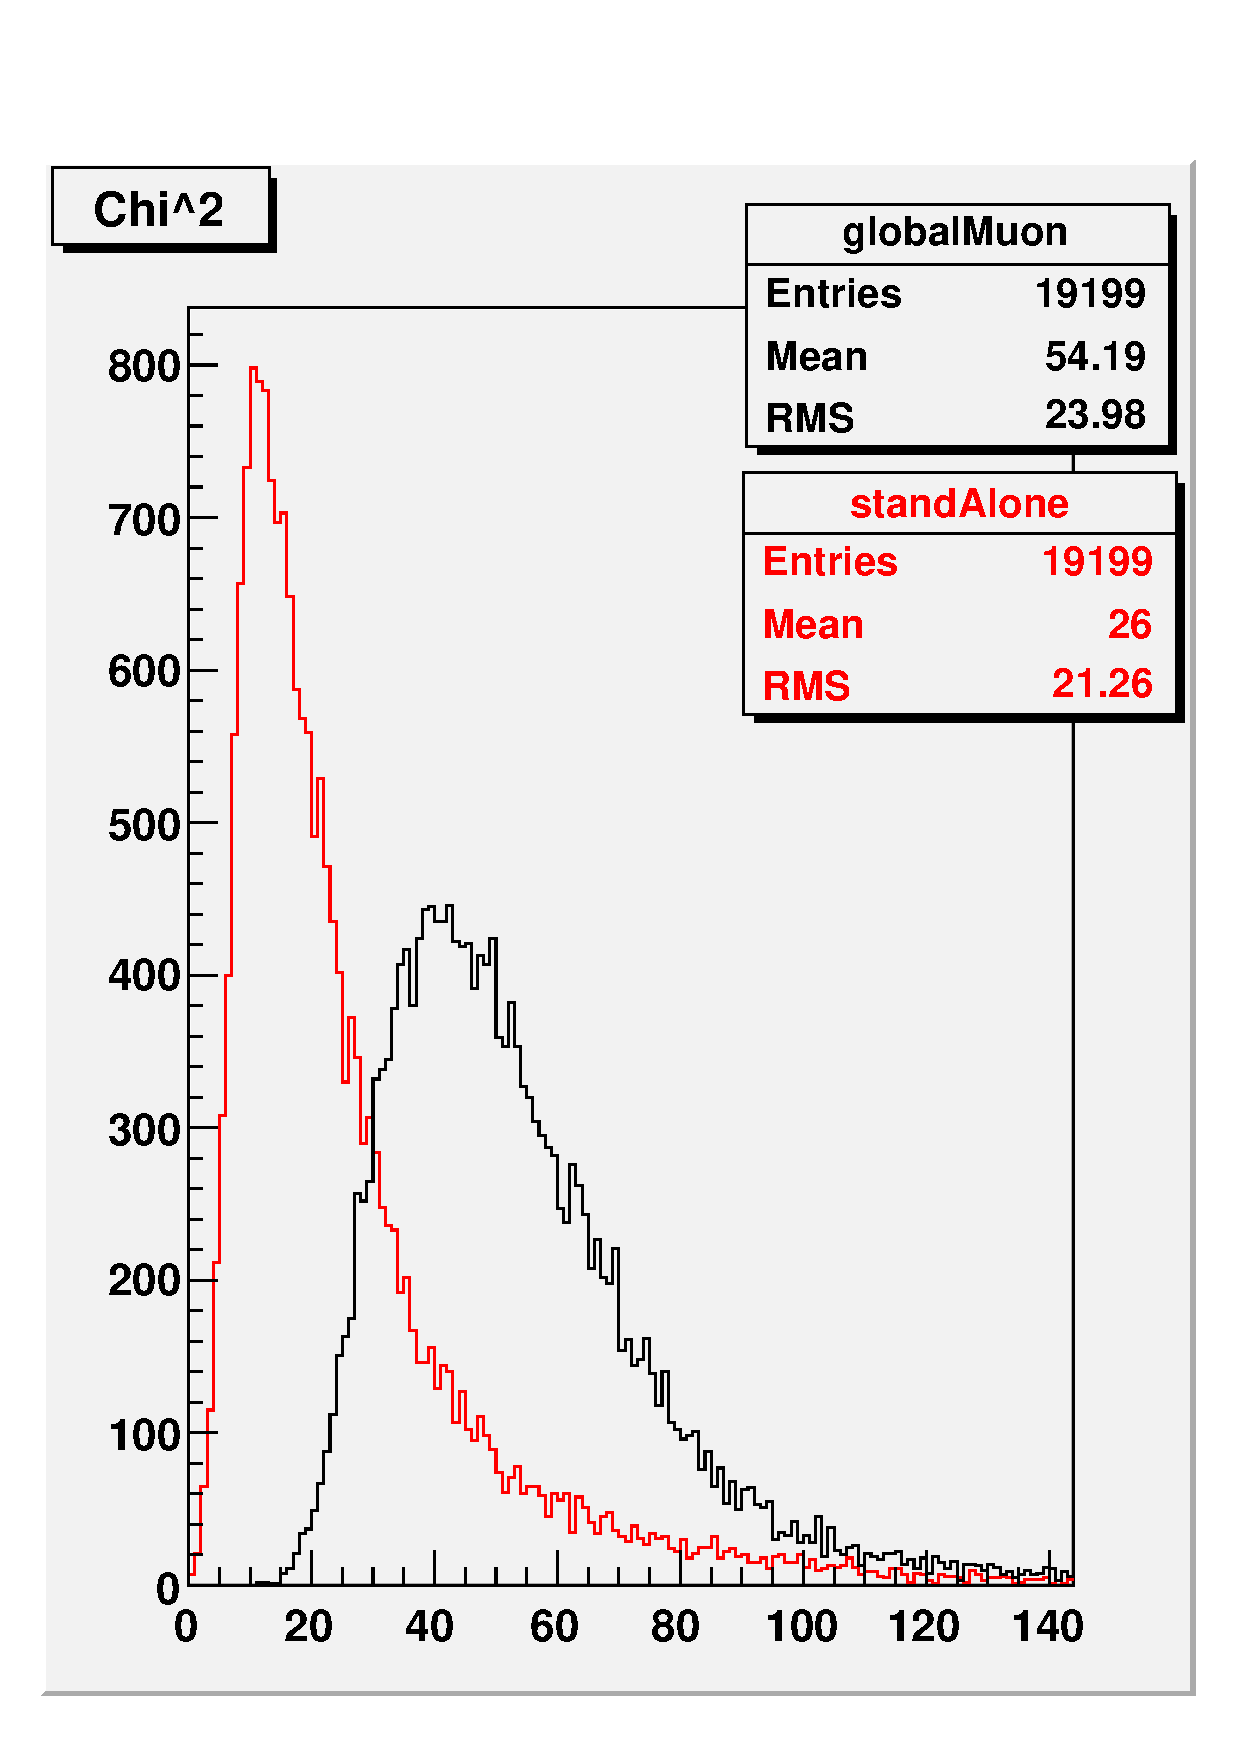
\includegraphics[width=0.5\linewidth]{chi2.pdf}
\end{frame}

\begin{frame}
\small

Other than being selected for large initial misalignment, these two
chambers are typical.  Most chambers show internal (layer-by-layer)
structure, presumably from miscalibration.

\begin{center}
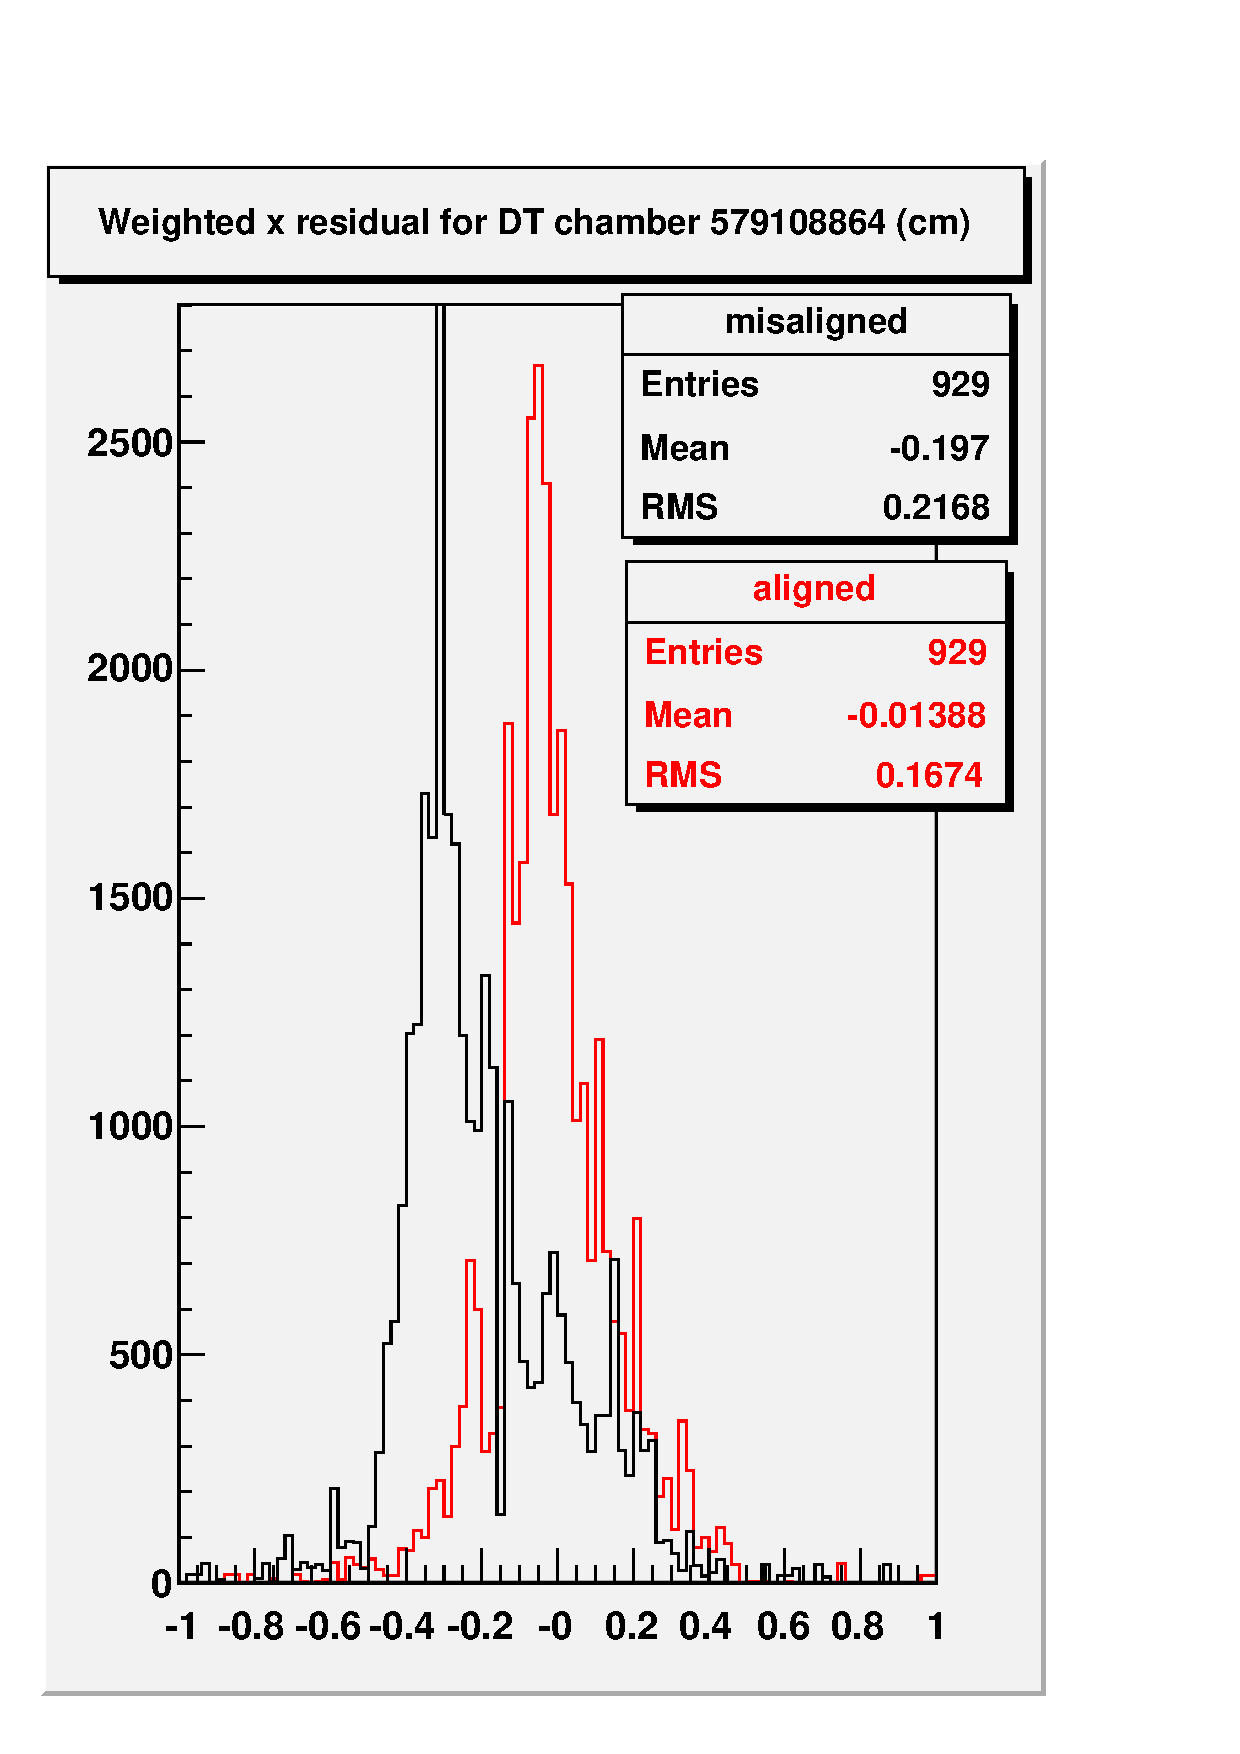
\includegraphics[width=0.4\linewidth]{chamberDT.pdf}
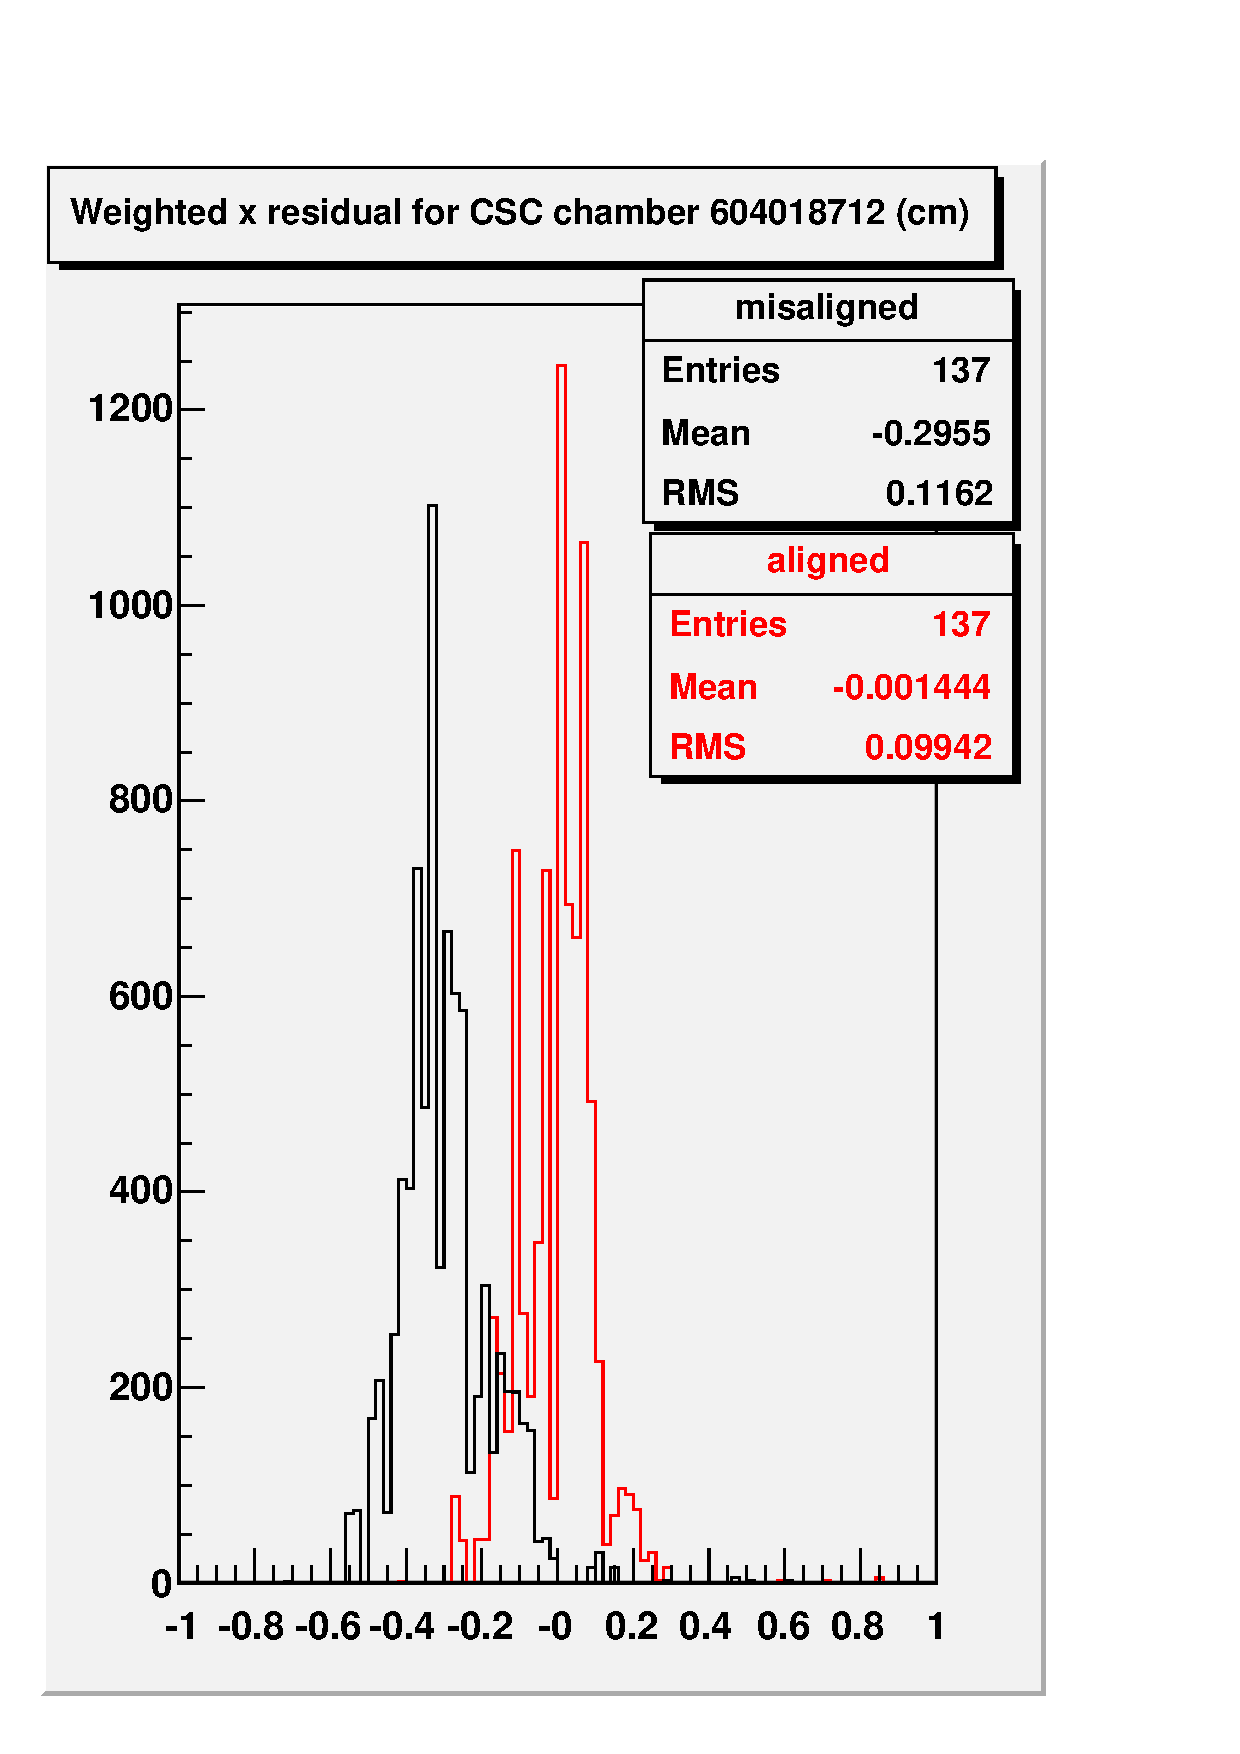
\includegraphics[width=0.4\linewidth]{chamberCSC.pdf}
\end{center}
\end{frame}

\begin{frame}
\small

(Looking at chamber-by-chamber residuals is a small step removed from
an iteration of HIP alignment.  So why not?)

\begin{center}
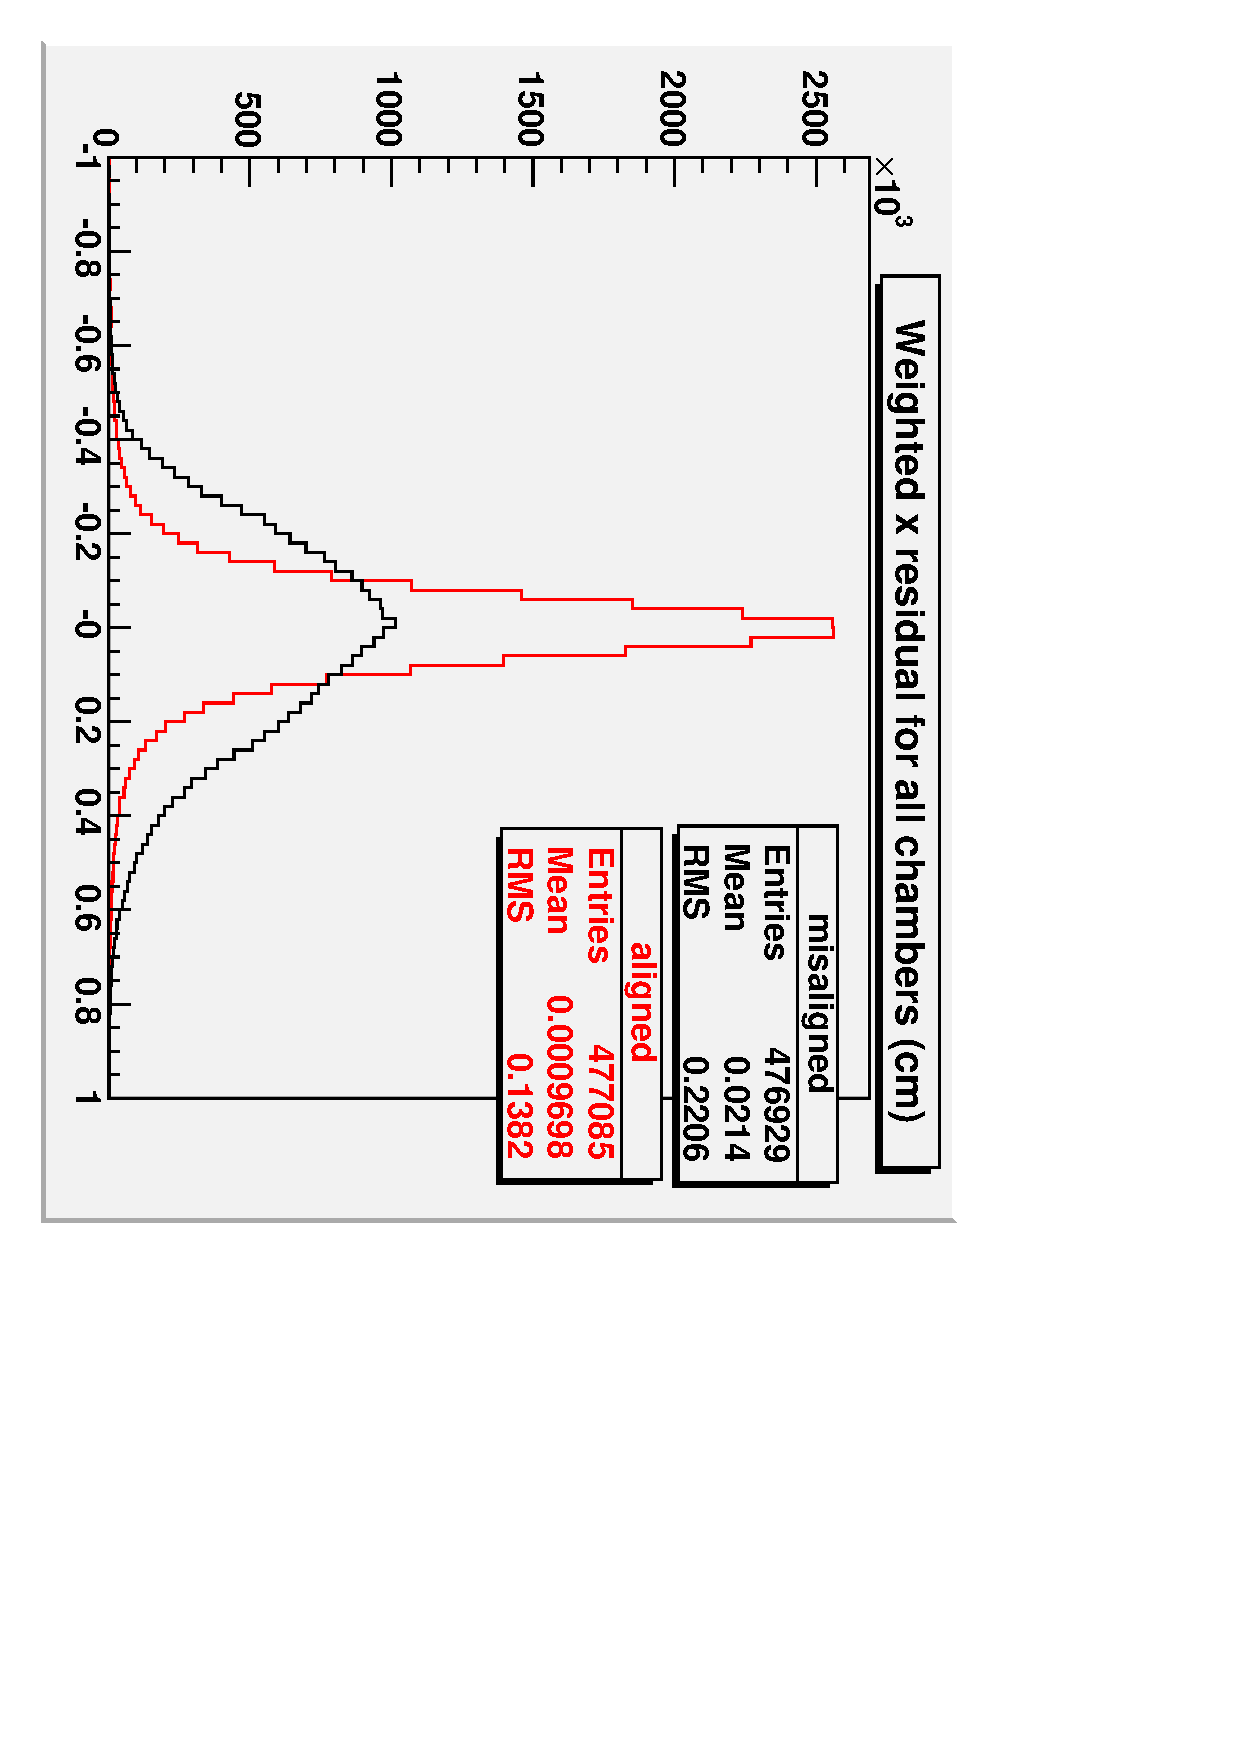
\includegraphics[height=0.8\linewidth, angle=90]{chambers.pdf}
\end{center}
\label{numpages}
\end{frame}

\end{document}
